\label{part_architecture}
\part{Application Architecture}

%%%%%%%%%%%%%%%%%%%%%%%%%%%%%%%%%%%%%%%%%%%%%%%%%%%%%%%%%%%%%%%%%%%%%%%%%%%
\begin{frame}
\frametitle{Application Architecture}
\framesubtitle{}
\begin{quote}
  ``Do what you would do anyway to build a highly scalable web application.''\\
  \hfill{}-- George Reese
\end{quote}
\end{frame}

%%%%%%%%%%%%%%%%%%%%%%%%%%%%%%%%%%%%%%%%%%%%%%%%%%%%%%%%%%%%%%%%%%%%%%%%%%%
\begin{frame}
\frametitle{Application Architecture}
\framesubtitle{Desaster Recovery}
\begin{itemize}
\item Plan for the worst, instances can and will fail
\item Automation, e.g. through contextualization and configuration management will help
  \begin{itemize}
  \item More on this later as part of contextualization
  \end{itemize}
  \item Particularly important when running user-facing services
\end{itemize}
\end{frame}



%%%%%%%%%%%%%%%%%%%%%%%%%%%%%%%%%%%%%%%%%%%%%%%%%%%%%%%%%%%%%%%%%%%%%%%%%%%
\begin{frame}
\frametitle{Compute and Data}
\framesubtitle{}
The cloud is not only about VM instances for processing. It is
also about data, storage, network, etc. Try and keep these concerns
separated.

Therefore:
\begin{itemize}
\item Avoid large data payloads in your VM images. Particularly, if
  the data is rather static and reused in more than one VM.
\item Make use of available storage resources such as block or object
  storage
  \begin{itemize}
  \item This will keep you away from the ``update trap''
  \item Software updates will not require re-distribution of all data
    contained in images
  \item Data updates can be managed centrally and also do not require
    re-distribution of large images
  \item Make use of the same data from multiple instances/images
  \end{itemize}
\end{itemize}
\end{frame}

%%%%%%%%%%%%%%%%%%%%%%%%%%%%%%%%%%%%%%%%%%%%%%%%%%%%%%%%%%%%%%%%%%%%%%%%%%%
\begin{frame}
\frametitle{Compute and Data}
\framesubtitle{Caching Example}
\begin{tikzpicture}
\node at (5,0) [overlay,absolute] {\pgfimage[width=.9\textwidth]{images/OM_Caching.png}};
\end{tikzpicture}
\end{frame}


%%%%%%%%%%%%%%%%%%%%%%%%%%%%%%%%%%%%%%%%%%%%%%%%%%%%%%%%%%%%%%%%%%%%%%%%%%%
\begin{frame}
\frametitle{Compute and Data}
%\framesubtitle{An Example}
An Example
\begin{itemize}
\item Create a generic VM containing the application and basic
  configuration, e.\,g. a MySQL server
\item Create a block storage template containing MySQL data directories
\item Modify MySQL startup scripts to wait for availability of block device
\end{itemize}
\begin{center}
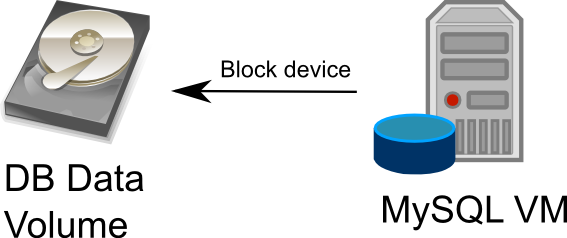
\includegraphics[width=.4\textwidth]{images/DBaaS.png}
\end{center}
\hfill\tiny Also mentioned in ``Cloud Application Architectures'' by George Reese
\end{frame}

%%%%%%%%%%%%%%%%%%%%%%%%%%%%%%%%%%%%%%%%%%%%%%%%%%%%%%%%%%%%%%%%%%%%%%%%%%%
\begin{frame}[fragile]
\frametitle{Compute and Data}
\framesubtitle{MySQL block device}
\begin{lstlisting}
# tree /mysql/
/mysql
|-- etc
|   `-- mysql
|       |-- conf.d
|       |   `-- mysqld_safe_syslog.cnf
|       |-- debian.cnf
|       |-- debian-start
|       |-- my.cnf
`-- mysql
\end{lstlisting}
The mysql service startup script has been modified to wait for the
/mysql mountpoint to come online. This requires the external block
device, e.\,g. \texttt{/dev/vdc}, to be mounted on that specific mount
point.
\end{frame}

%%% Local Variables:
%%% TeX-master: "2014-05-23_Best_Practices"
%%% End:
